\section*{Задание 2}
    Разложить функцию $ f(x) = x (1-x) ^4 $ в ряд Фурье по собственным функциям $ y_k $. Построить графики функции и ряда Фурье для пяти гармоник.

    Поскольку система нормированная, то
    \[ C_k = \frac{(f, y_k)}{(y_k, y_k)} = (f, y_k) = \int_0^1 \left( x (1-x) ^4 \cdot \sqrt{2} \sin \left( (0.5 + k) \pi x \right) \right) dx \]

    Посчитаем первые 5 коэффициентов:

    \begin{center}

        \begin{tabular}{|c|c|c|c|c|c|}
            \hline
            $ k $ & 0 & 1 & 2 & 3 & 4 \\
            \hline
            $ C_k $& $0.01975 \dots$& $0.03419 \dots$ & $0.01953 \dots$ & $0.00756 \dots$ & $0.00378 \dots$\\
            \hline
        \end{tabular}

    \end{center}
    \[
        f(x) = \sum_{k=0}^4 \left( C_k \cdot \sqrt{2} \sin \left( (0.5 + k) \pi x \right) \right)
    \]
    \begin{figure}[H]
        \centering
        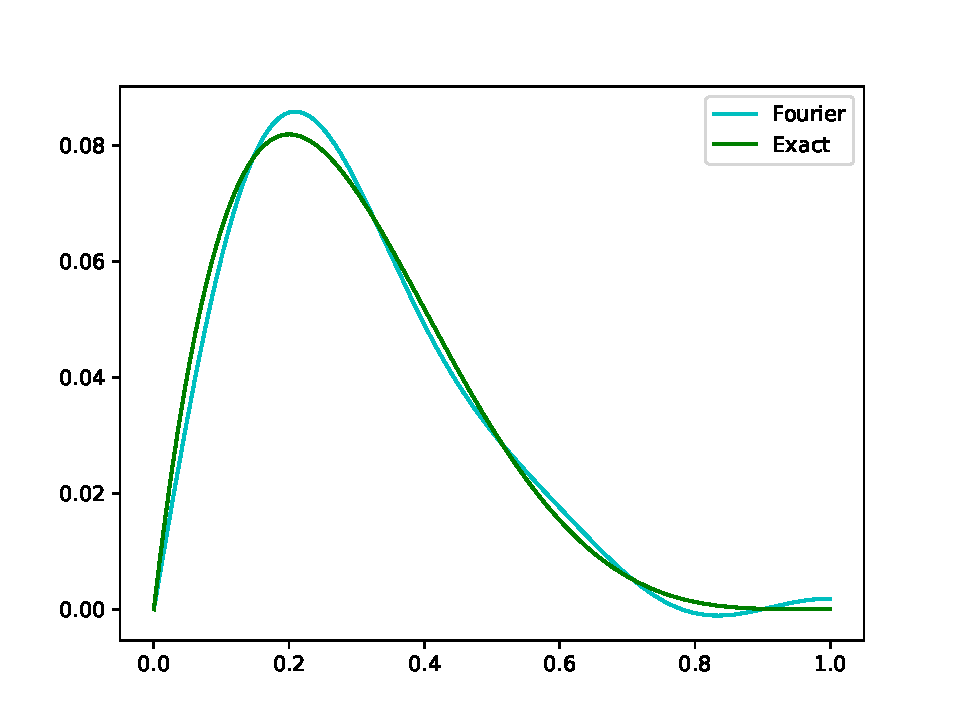
\includegraphics[width=14cm]{fourier.pdf}
    \end{figure}
